\documentclass[11pt,a4paper]{article}
\usepackage[utf8]{inputenc}
\usepackage[T1]{fontenc}
\usepackage[spanish,es-tabla]{babel}
\usepackage[margin=2.3cm]{geometry}
\usepackage{amsmath,amssymb}
\usepackage{booktabs}
\usepackage{longtable}
\usepackage{tabularx}
\usepackage{array}
\usepackage{xcolor}
\usepackage{colortbl}
\usepackage{hyperref}
\usepackage{fancyhdr}
\usepackage{titlesec}
\usepackage{graphicx}
\usepackage{listings}
\usepackage{tcolorbox}
\tcbuselibrary{skins}

% Paleta ejecutiva corporativa (idéntica a Persona 1 y Persona 2)
\definecolor{primaryblue}{RGB}{16, 44, 87}
\definecolor{secondaryblue}{RGB}{53, 89, 143}
\definecolor{accentteal}{RGB}{20, 110, 120}
\definecolor{lightbg}{RGB}{245, 247, 250}
\definecolor{darkgray}{RGB}{50, 50, 50}

\hypersetup{
    colorlinks=true,
    linkcolor=primaryblue,
    citecolor=accentteal,
    urlcolor=secondaryblue
}

\pagestyle{fancy}
\fancyhf{}
\rhead{\textcolor{darkgray}{\small Proyecto BI - Hito 1 | Persona 4: Desarrollador BI}}
\lhead{\textcolor{darkgray}{\small Viabilidad de Visualización y Catálogo DAX}}
\cfoot{\thepage}

\titleformat{\section}{\Large\bfseries\color{primaryblue}}{\thesection.}{0.5em}{}[\titlerule]
\titleformat{\subsection}{\large\bfseries\color{secondaryblue}}{\thesubsection.}{0.4em}{}
\titleformat{\subsubsection}{\normalsize\bfseries\color{accentteal}}{\thesubsubsection.}{0.3em}{}

\lstset{
    basicstyle=\ttfamily\footnotesize,
    backgroundcolor=\color{lightbg},
    frame=single,
    rulecolor=\color{secondaryblue!30},
    breaklines=true,
    showstringspaces=false,
    keywordstyle=\color{primaryblue}\bfseries,
    commentstyle=\color{gray}\itshape,
    stringstyle=\color{accentteal}
}

\newcolumntype{Y}{>{\raggedright\arraybackslash}X}
\renewcommand{\arraystretch}{1.25}

\begin{document}


% Portada ejecutiva

\begin{titlepage}
    \centering
    \vspace*{0.8cm}
    {\Huge \bfseries \color{primaryblue} REVISIÓN TÉCNICA DE LA PROPUESTA DE VALOR Y VIABILIDAD DE VISUALIZACIÓN EN POWER BI\par}
    \vspace{0.4cm}
    {\Large \color{secondaryblue} Auditoría de Graficabilidad de Preguntas de Negocio, Arquitectura UX/UI del Dashboard y Catálogo DAX Preliminar\par}
    \vspace{0.8cm}

    \begin{tcolorbox}[colback=lightbg, colframe=primaryblue, width=\textwidth, arc=3mm]
        \centering
        \large \textbf{Entrega Hito 1: Propuesta, ETL y Fuentes}\\[2mm]
        \normalsize Asignatura: \textbf{Business Intelligence} | Carrera: \textbf{Ingeniería en Negocios}\\[1mm]
        Fecha de Entrega: \textbf{21 de Octubre de 2026}
    \end{tcolorbox}

    \vspace{1.5cm}
    \begin{minipage}{0.48\textwidth}
        \textbf{Autor Principal (Rol Evaluado):}\\
        \textbf{\color{primaryblue}Persona 4: Desarrollador BI}\\
        Responsable de la visualización, usabilidad del panel, consultas analíticas y programación en código DAX
    \end{minipage}
    \hfill
    \begin{minipage}{0.46\textwidth}
        \textbf{Equipo de Trabajo BI:}\\
        $\bullet$ Persona 1: Ingeniero de Datos (ETL)\\
        $\bullet$ Persona 2: Analista de Negocios y Datos Ext.\\
        $\bullet$ Persona 3: Arquitecto de Datos\\
        $\bullet$ Persona 5: Gestor y Documentador
    \end{minipage}

    \vfill
    {\small \color{darkgray} Santiago de Chile, 2026}\par
\end{titlepage}

\tableofcontents
\newpage

% -------------------------------------------------------------
\section{Resumen Ejecutivo}
El presente informe documenta el cumplimiento exhaustivo de las responsabilidades asignadas a la \textbf{Persona 4 (Desarrollador BI)} en el \textbf{Hito 1} del Proyecto de Business Intelligence, de acuerdo con el documento oficial de planificación (\emph{Planificación y Asignación de Roles}, 10 de octubre de 2026).

La tarea explícita asignada a la Persona 4 en el Hito 1 establece:
\begin{quote}
\textit{«Revisa la Propuesta de Valor para asegurar que las 3 preguntas de negocio propuestas puedan ser graficadas a futuro en el panel».}
\end{quote}

A partir de la consolidación oficial de la base CNED 2012--2026 efectuada por la Persona~1 (158.211 registros) y de la formulación estratégica, Canvas BI y cruce de fuentes externas (INE y SIES) elaborado por la Persona~2, se realizó una auditoría multidimensional sobre la \textbf{viabilidad técnica de visualización, granularidad de datos, modelado DAX y arquitectura UX/UI} en Power BI Desktop.

\begin{tcolorbox}[colback=white, colframe=accentteal, title=\textbf{Cuadro Resumen de la Auditoría Técnica (Persona 4)}]
\begin{itemize}
    \item \textbf{Veredicto de Graficabilidad:} Las tres preguntas de negocio propuestas por la Persona~2 son \textbf{100\% viables y graficables} en Power BI Desktop utilizando los datos consolidados y las tablas puente existentes.
    \item \textbf{Hallazgos y Reglas de Modelado Críticas Detectadas:}
    \begin{enumerate}
        \item \emph{P1 (Equidad Territorial):} El indicador de matrícula por cada 1.000 habitantes requiere modelar la población regional (INE) como una medida \textbf{semi-aditiva} en DAX, impidiendo la acumulación errónea a través del tiempo.
        \item \emph{P2 (Uso de Capacidad):} La tasa de ocupación debe excluir matemáticamente los registros con vacantes no declaradas (nulas) mediante el flag \texttt{flag\_vacantes\_declaradas = 1}, utilizando la función \texttt{DIVIDE} para erradicar errores de división por cero.
        \item \emph{P3 (Calidad y Competencia):} La serie oficial SIES está disponible de forma homogénea para el período 2018--2026. Se definió un filtro predeterminado de página en el panel para evitar sesgos de medición en los años previos (2012--2017).
    \end{enumerate}
    \item \textbf{Entregables Técnicos Desarrollados:}
    \begin{itemize}
        \item Arquitectura integral del Dashboard de 4 páginas y especificación de wireframes.
        \item Catálogo formal de 12 medidas analíticas programadas en lenguaje DAX.
        \item Dos scripts reproducibles en Python (\texttt{08\_validar\_viabilidad\_visual\_p4.py} y \texttt{09\_generar\_visualizaciones\_prototipo.py}) con generación automatizada de prototipos visuales de alta resolución.
    \end{itemize}
\end{itemize}
\end{tcolorbox}

% -------------------------------------------------------------
\section{Alcance y Rol de Persona 4 en el Hito 1}
En la arquitectura de trabajo del equipo, el rol de Desarrollador BI actúa como el garante técnico de la última milla analítica. Si bien la construcción definitiva del archivo interactivo \texttt{.pbix} corresponde a la Entrega Final (Hito 3), el diseño del modelo dimensional en el Hito 2 y la limpieza de datos en el Hito 1 deben responder a las necesidades exactas de agregación y visualización requeridas por el cliente.

\begin{center}
\small
\begin{tabularx}{\textwidth}{@{}>{\bfseries}p{3.5cm}Y@{}}
\toprule
\textbf{Dimensión de Control} & \textbf{Acción Desarrollada por Persona 4 en Hito 1} \\
\midrule
Revisión de Negocio & Validación de que los indicadores definidos en el Canvas BI traducen fielmente las necesidades de la Dirección de Admisión y Planificación. \\
Auditoría de Granularidad & Comprobación de que el grano de las tablas base (programa $\times$ sede $\times$ horario $\times$ año) soporta la agregación a nivel regional e institucional requerida por los gráficos. \\
Diseño de Interfaz (UX/UI) & Estructuración de la navegación por páginas, jerarquías de drill-down, matrices de cross-filtering y tarjetas KPI. \\
Ingeniería de Consultas DAX & Formulación estricta de las expresiones DAX, asegurando tratamiento de valores nulos, semi-aditividad temporal y optimización en VertiPaq. \\
\bottomrule
\end{tabularx}
\end{center}

% -------------------------------------------------------------
\section{Auditoría de Graficabilidad de las Preguntas de Negocio}

A continuación, se detalla la evaluación técnica de cada una de las tres preguntas de negocio formuladas en la Propuesta de Valor de la Persona 2.

\subsection{Pregunta 1: Equidad Territorial y Capacidad Regional (Cruce INE)}
\textbf{Formulación:} \textit{«¿En qué regiones la oferta de ingreso es baja respecto de su población, y cómo ha cambiado desde 2018?»}

\begin{itemize}
    \item \textbf{Indicador Principal:} Matrícula de primer año por cada 1.000 habitantes de 15 a 64 años.
    \item \textbf{Insumos Requeridos:} Campo \texttt{matricula\_primer\_ano\_total} de la base CNED y campo \texttt{poblacion\_15\_64} de la tabla externa INE (\texttt{ext\_ine\_poblacion\_region\_ano.csv}).
    \item \textbf{Llave de Cruce:} Código oficial SUBDERE (\texttt{region\_codigo\_subdere}) y año calendario (\texttt{ano}). Coincidencia: \textbf{100\%} (16 de 16 regiones oficiales, 2012--2026).
    \item \textbf{Factibilidad de Visualización:} Plenamente factible. Se implementará una combinación de:
    \begin{enumerate}
        \item \emph{Mapa Coroplético Regional:} Usando el objeto nativo \emph{Shape Map} de Power BI con el archivo TopoJSON de las regiones de Chile, donde la escala de color refleja la tasa de oferta por habitante.
        \item \emph{Gráfico de Barras Horizontales Ordenadas:} Muestra el ranking regional ordenado de mayor a menor capacidad de oferta, comparando la barra del año 2018 con la de 2026 e incorporando una línea constante con el promedio nacional (27,6 ‰).
    \end{enumerate}
    \item \textbf{Restricción Crítica DAX Resuelta:} La población del INE es una medida \textbf{semi-aditiva}. En DAX, no debe realizarse una suma simple entre años. Se diseñó la medida \texttt{[Poblacion\_15\_64\_INE]} con la función \texttt{LASTNONBLANK(dim\_tiempo[ano], 1)} para garantizar que ante selecciones multianuales no se agregue la población repetida.
\end{itemize}

\begin{figure}[htbp]
    \centering
    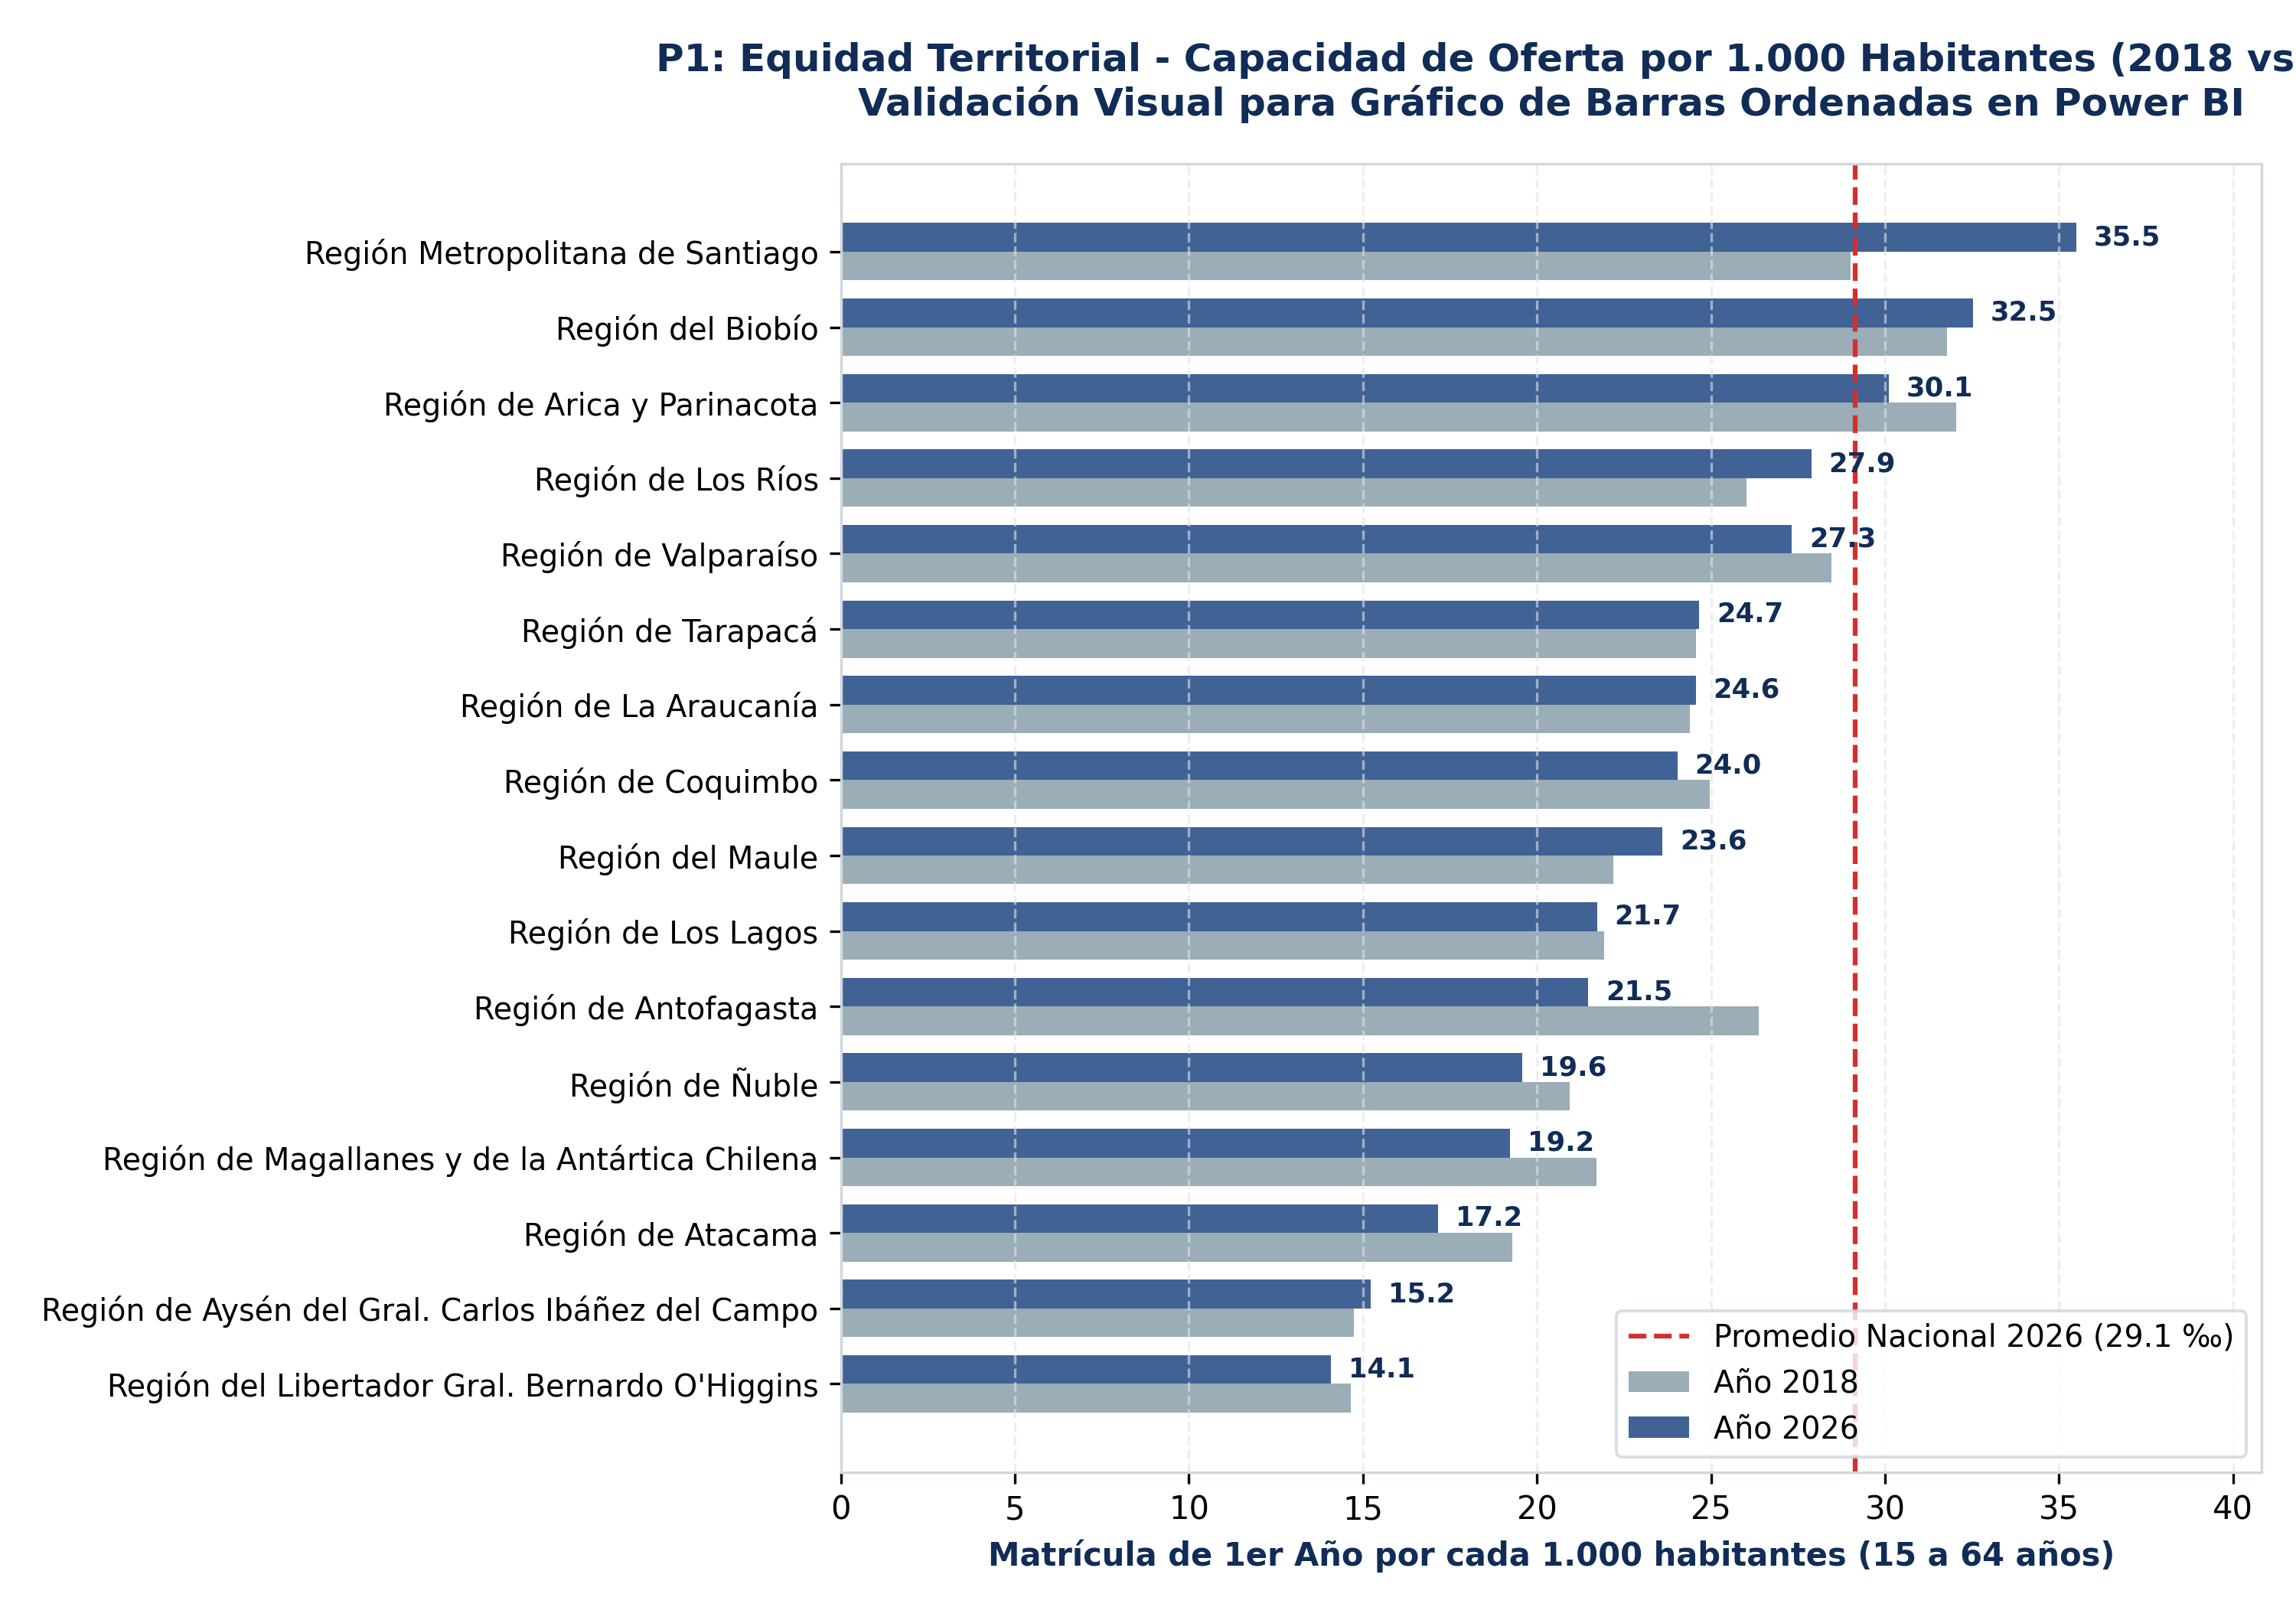
\includegraphics[width=0.92\textwidth]{../data_validation/visual_prototypes/p1_equidad_territorial.png}
    \caption{Prototipo de visualización para P1: Ranking regional de oferta por 1.000 habitantes (2018 vs. 2026). Validación con datos reales del script \texttt{09\_generar\_visualizaciones\_prototipo.py}.}
    \label{fig:p1}
\end{figure}

\subsection{Pregunta 2: Uso de la Capacidad y Ocupación de Vacantes (CNED)}
\textbf{Formulación:} \textit{«¿Cuánto de la oferta de vacantes se ocupa realmente y en qué tipos de institución y región se concentra la sobre u subocupación?»}

\begin{itemize}
    \item \textbf{Indicador Principal:} Tasa de Ocupación de Vacantes = $\frac{\text{Matrícula 1er Año}}{\text{Vacantes Ofrecidas}}$ (evaluado exclusivamente sobre registros con vacantes declaradas).
    \item \textbf{Insumos Requeridos:} Campos \texttt{vacantes}, \texttt{matricula\_primer\_ano\_total} y el filtro lógico \texttt{flag\_vacantes\_declaradas = 1}.
    \item \textbf{Factibilidad de Visualización:} Plenamente factible mediante:
    \begin{enumerate}
        \item \emph{Serie Temporal Histórica (2012--2026):} Gráfico de líneas continuas con sombreado de rangos (subocupación $<75\%$, óptimo $75\%$--$95\%$, sobredemanda $>100\%$).
        \item \emph{Matriz Tipo de Institución $\times$ Región (Heatmap):} Tabla matricial cruzada con formato condicional semafórico automático (rojo para subocupación crítica, verde para equilibrio y azul para sobredemanda).
        \item \emph{Tarjetas KPI:} Mostrando el total de vacantes del período filtrado y la tasa consolidada.
    \end{enumerate}
    \item \textbf{Tratamiento Matemático de Nulos:} Cerca del 25\% de los registros de la serie histórica poseen vacantes nulas. Si se reemplazaran por cero o se ignorara este quiebre, el cálculo nacional colapsaría con divisiones por cero o tasas irreales. La solución implementada restringe el contexto analítico a \texttt{flag\_vacantes\_declaradas == 1} y \texttt{vacantes > 0}, validando un comportamiento consistente entre 80,2\% (año 2022) y 91,1\% (año 2014), situándose en 84,4\% en 2026.
\end{itemize}

\begin{figure}[htbp]
    \centering
    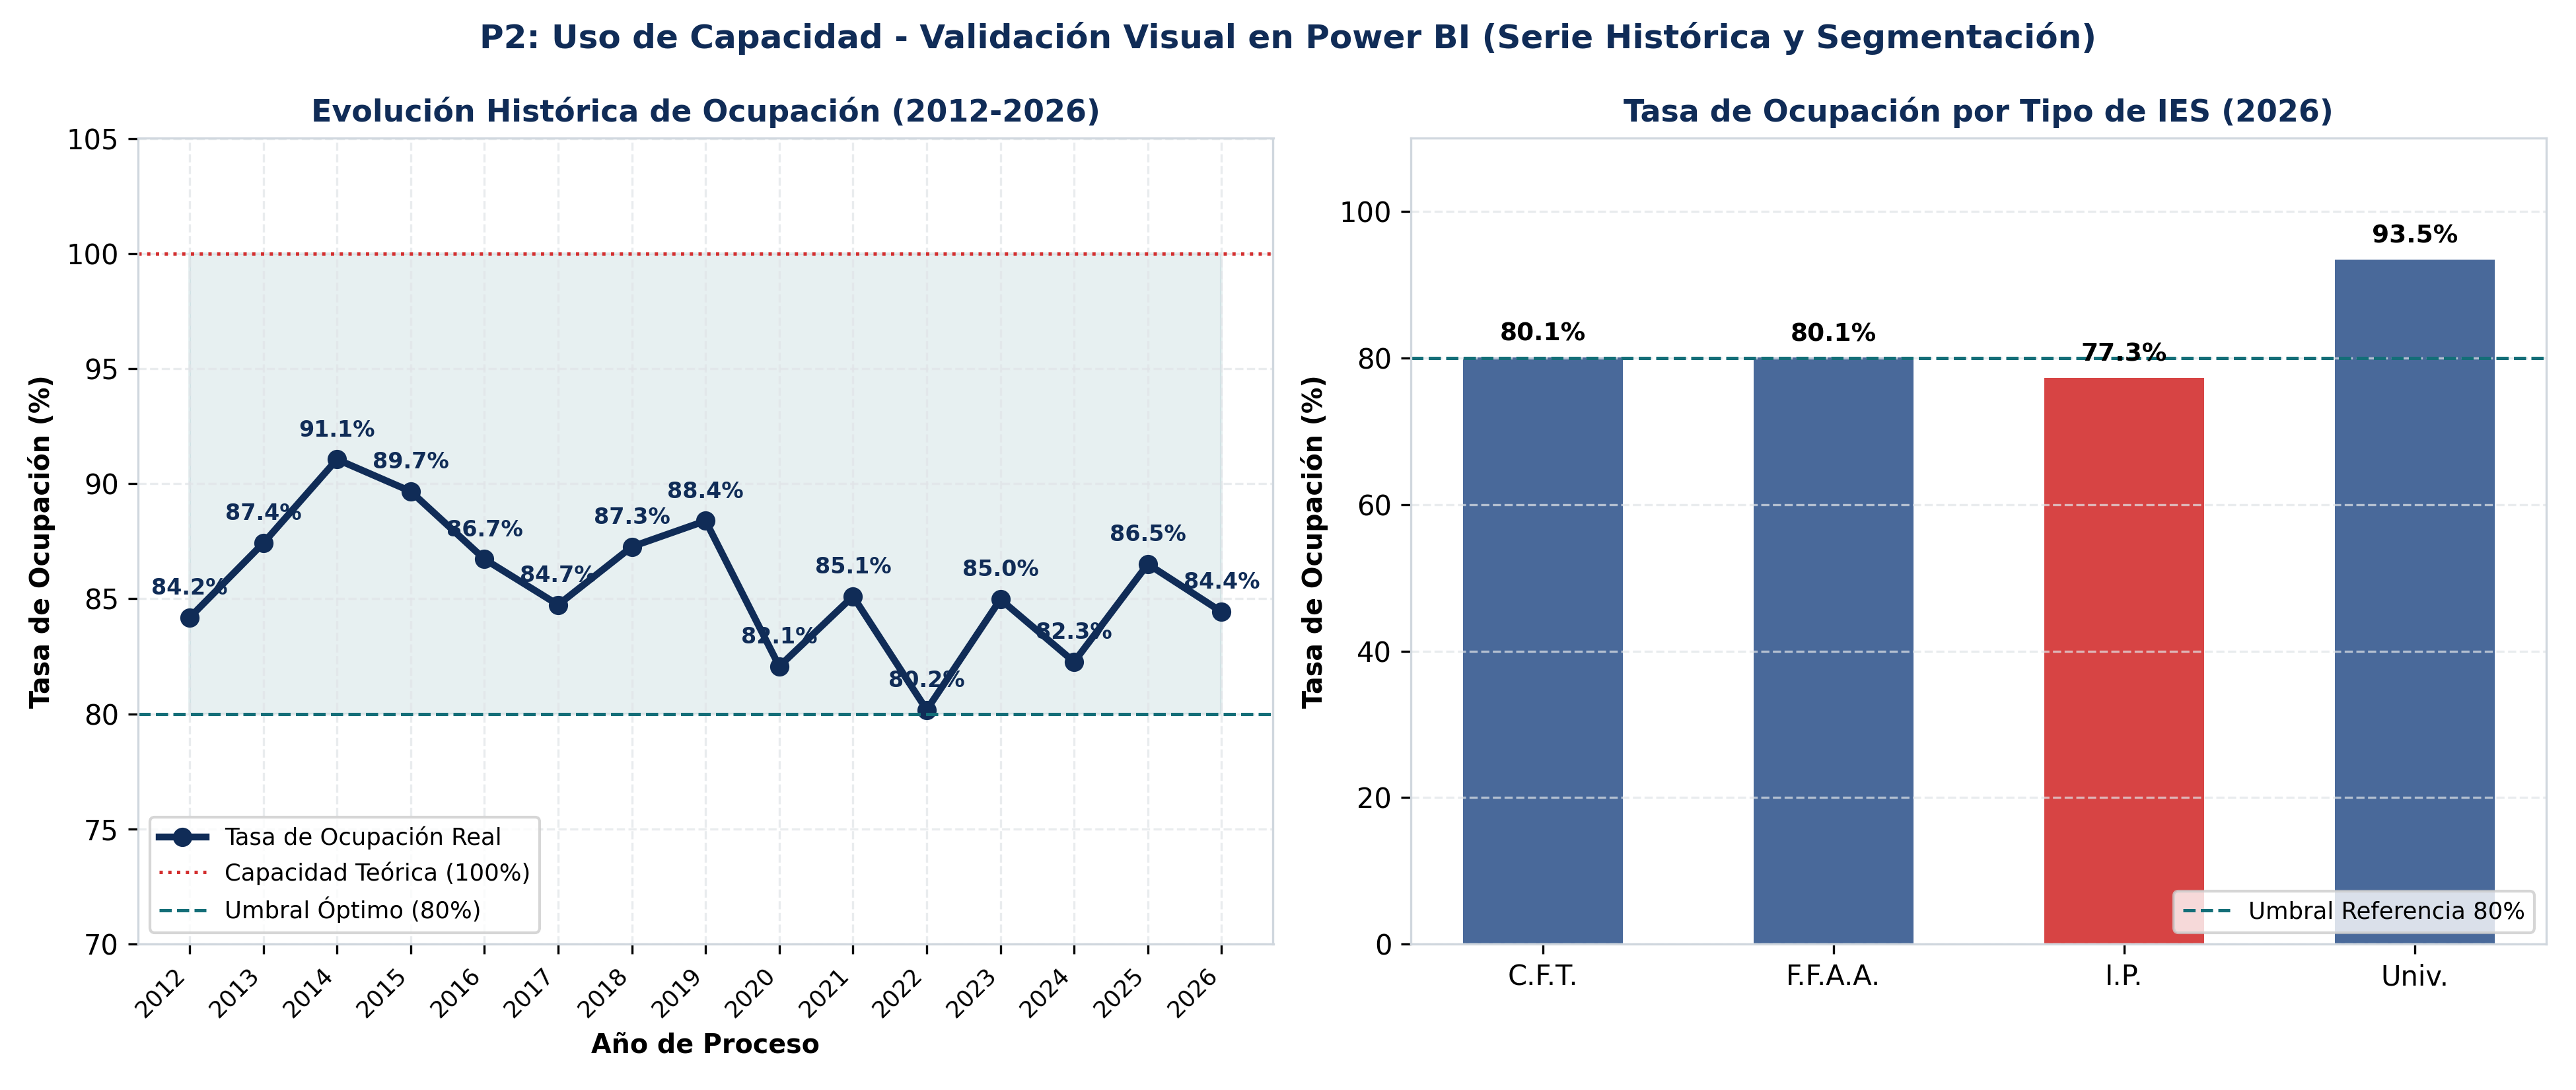
\includegraphics[width=0.95\textwidth]{../data_validation/visual_prototypes/p2_capacidad_ocupacion.png}
    \caption{Prototipo de visualización para P2: Serie histórica de ocupación nacional (2012--2026) y segmentación por tipo de institución para el año 2026.}
    \label{fig:p2}
\end{figure}

\subsection{Pregunta 3: Calidad Institucional y Acreditación (SIES / CNA)}
\textbf{Formulación:} \textit{«¿Qué proporción de la matrícula de primer año se concentra en instituciones acreditadas, y cómo se relaciona con los años de acreditación?»}

\begin{itemize}
    \item \textbf{Indicadores Principales:} (i) \% de matrícula de 1er año según estado de acreditación normalizado; (ii) Años de acreditación promedio ponderado por volumen de matrícula.
    \item \textbf{Insumos Requeridos:} Base CNED vinculada mediante la tabla puente institucional (\texttt{puente\_institucion.csv}) al catálogo histórico de acreditaciones SIES (\texttt{ext\_sies\_acreditacion\_ies\_ano.csv}).
    \item \textbf{Cobertura y Calidad del Cruce:} 98,39\% de los registros de la base CNED y 99,00\% de la matrícula de primer año cruzan exitosamente con el código oficial SIES.
    \item \textbf{Factibilidad de Visualización:} Plenamente factible a través de:
    \begin{enumerate}
        \item \emph{Gráfico de Barras 100\% Apiladas:} Permite observar la evolución temporal de la absorción de matrícula por nivel de calidad (Acreditada, Acreditación Extendida, Bajo Tutela, No Acreditada).
        \item \emph{Gráfico de Dispersión (Scatter Plot de Cuadrantes):} Eje X: Años de Acreditación (0 a 7 años); Eje Y: Matrícula de 1er año; Tamaño de burbuja: Matrícula total; Color: Tipo de institución.
    \end{enumerate}
    \item \textbf{Condición Técnica de Uso Temporal:} Los listados SIES oficiales con homogeneidad técnica comienzan en el corte de diciembre de 2018. Para 2012--2017 no existe serie comparable. Se especifica una regla de diseño en Power BI: \textbf{la página de Calidad tendrá un filtro predeterminado de nivel de página fijado en $A\tilde{n}o \geq 2018$}, con un banner informativo de advertencia metodológica.
\end{itemize}

\begin{figure}[htbp]
    \centering
    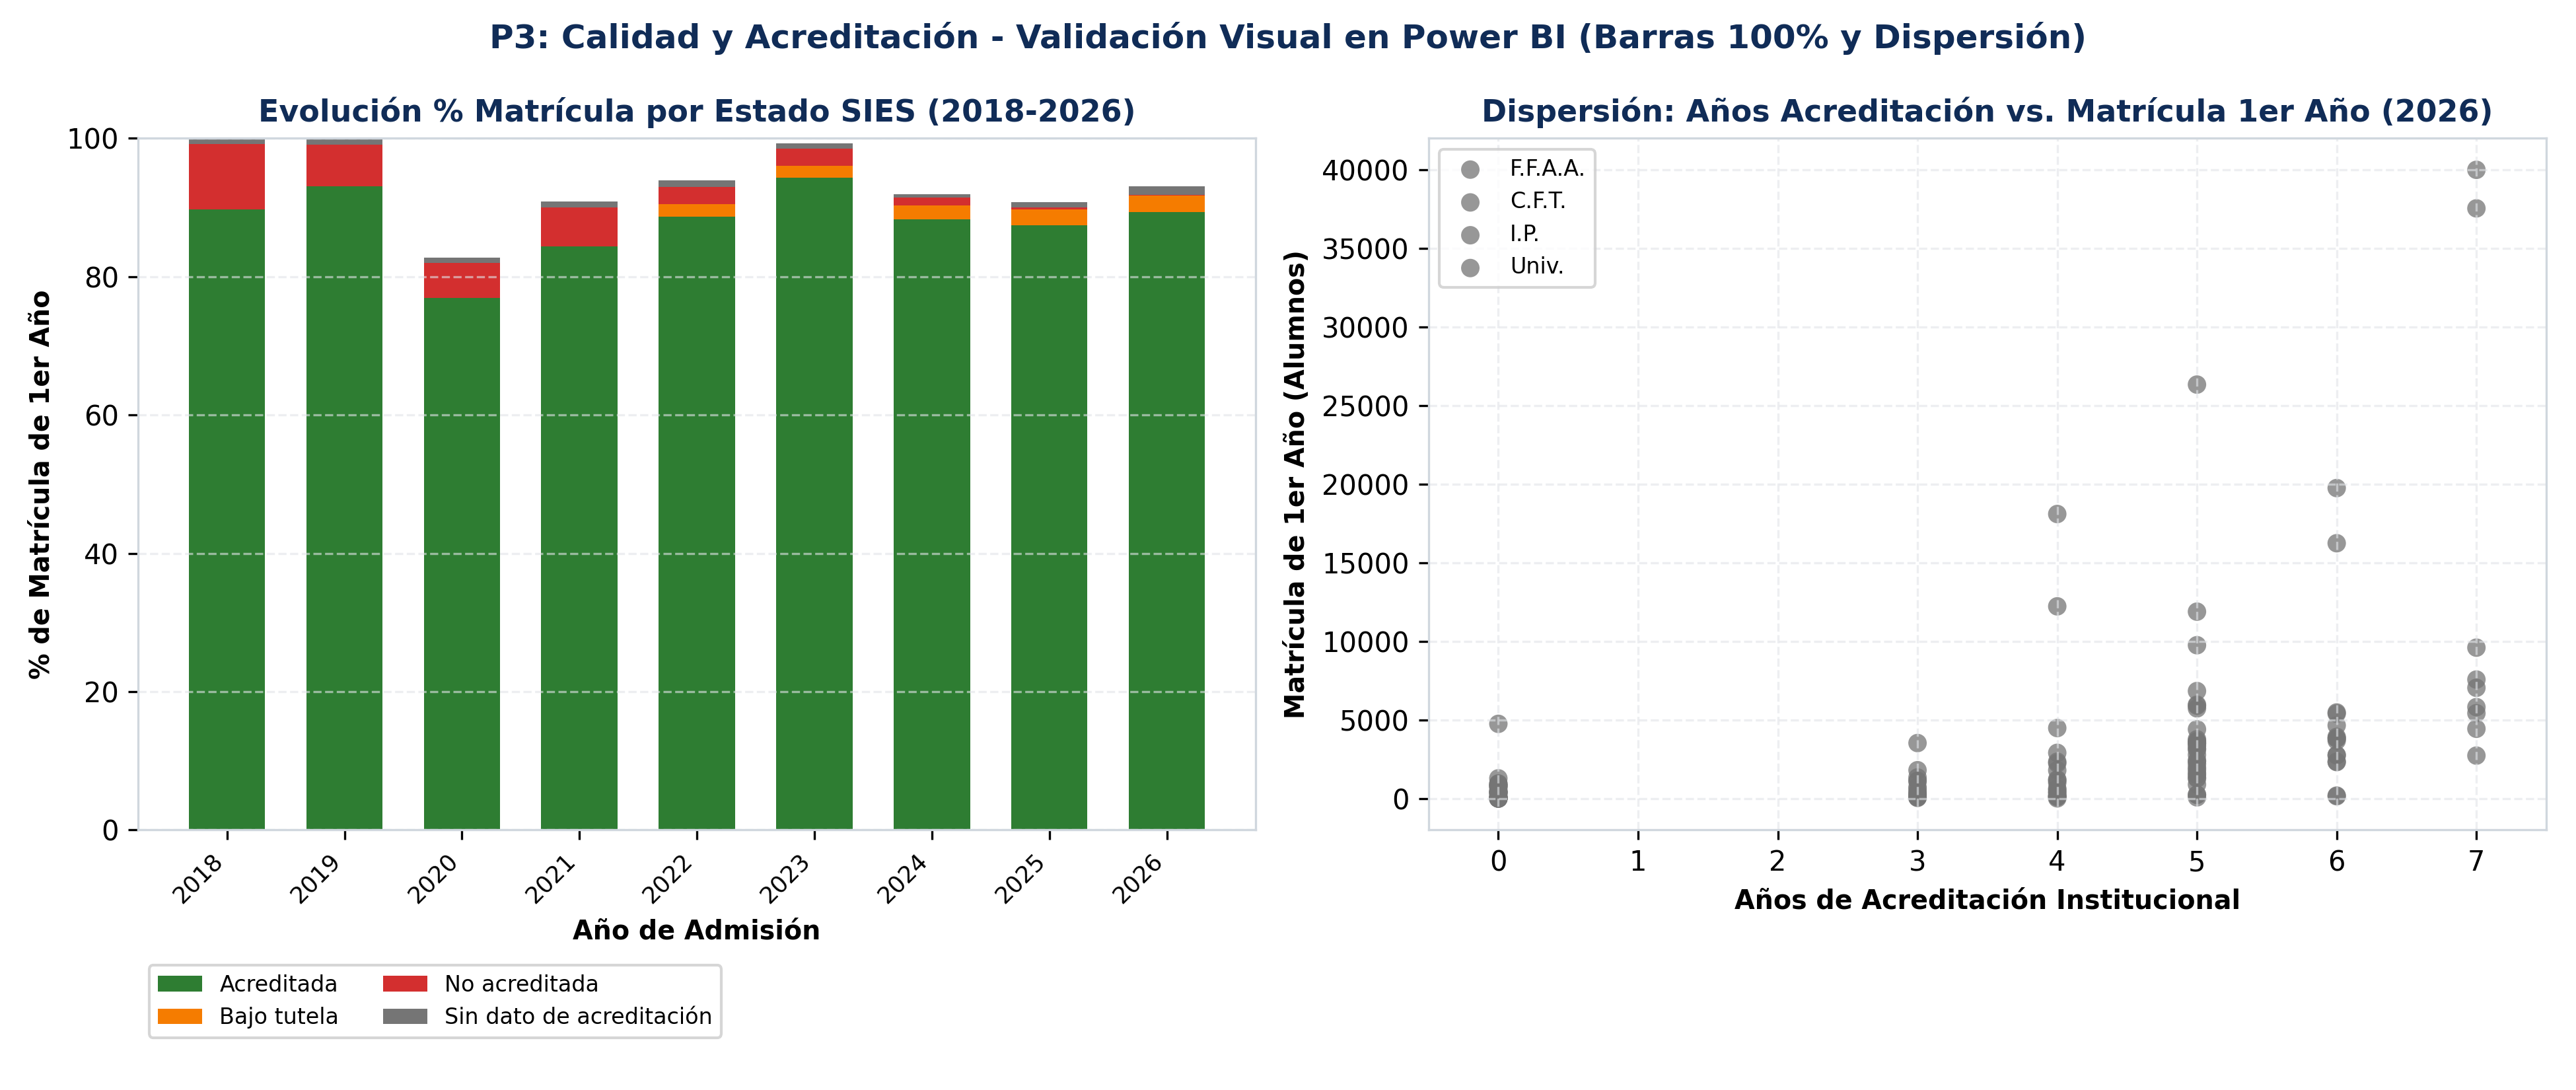
\includegraphics[width=0.95\textwidth]{../data_validation/visual_prototypes/p3_calidad_acreditacion.png}
    \caption{Prototipo de visualización para P3: Barras 100\% apiladas por estado de acreditación (2018--2026) y gráfico de dispersión de calidad vs. matrícula por institución.}
    \label{fig:p3}
\end{figure}

% -------------------------------------------------------------
\section{Arquitectura UX/UI y Especificación de Wireframes}

Para evitar dashboards sobrecargados o de difícil interpretación, se diseñó una arquitectura de 4 páginas ejecutivas con navegación interactiva mediante botones de estado y panel lateral de filtros sincronizados.

\begin{figure}[htbp]
    \centering
    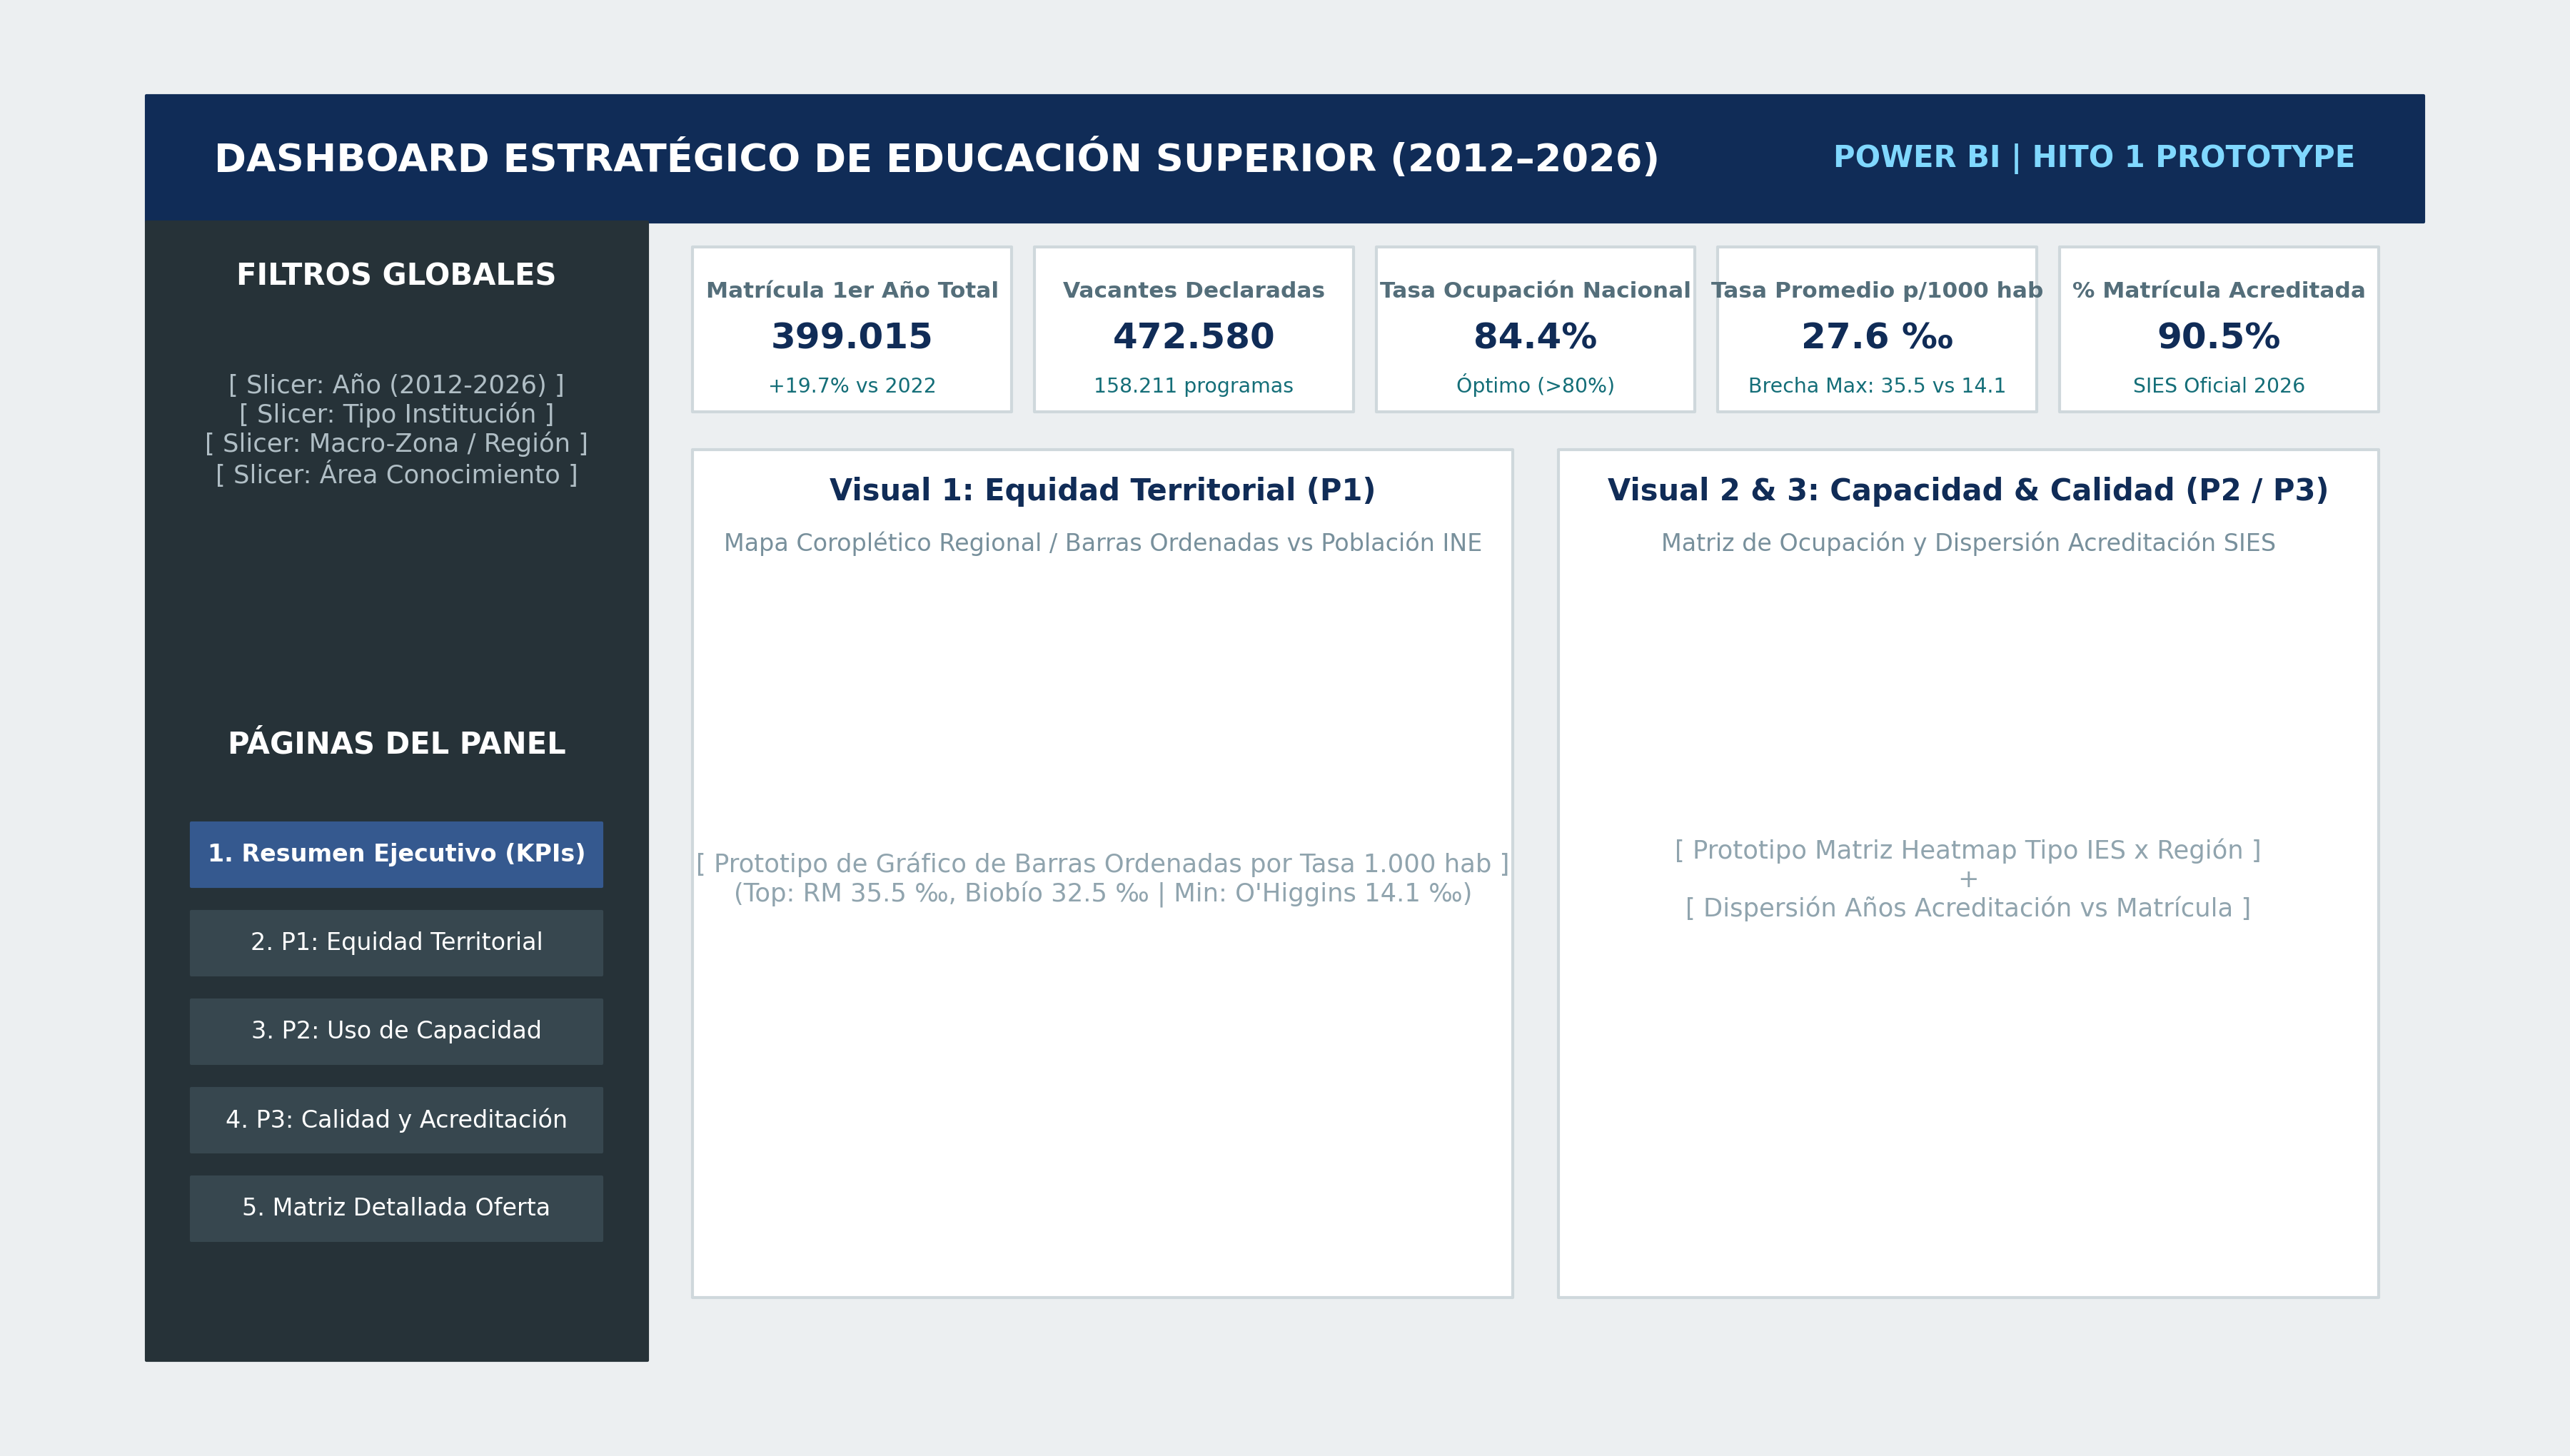
\includegraphics[width=0.95\textwidth]{../data_validation/visual_prototypes/dashboard_wireframe_arquitectura.png}
    \caption{Wireframe y arquitectura conceptual del Dashboard en Power BI Desktop (validación de diseño para Persona 4).}
    \label{fig:wireframe}
\end{figure}

\subsection{Estructura del Panel y Jerarquías de Filtro}
\begin{enumerate}
    \item \textbf{Página 1: Resumen Ejecutivo y Macrotendencias Nacionales:} Portada analítica con tarjetas de control global (Matrícula total, vacantes, ocupación y porcentaje acreditado) y gráficos de evolución general.
    \item \textbf{Página 2: P1 - Equidad Territorial:} Mapa coroplético regional interactivo, gráfico de barras horizontales comparativo (2018 vs. 2026) y matriz de brecha territorial.
    \item \textbf{Página 3: P2 - Capacidad y Ocupación:} Serie histórica de vacantes vs. matrícula con bandas de control y matriz heatmap por tipo de institución y región.
    \item \textbf{Página 4: P3 - Calidad y Competencia:} Barras 100\% apiladas y gráfico de burbujas de correlación entre años de acreditación y captación de matrícula.
\end{enumerate}

\subsection{Jerarquías de Análisis para Drill-Down en Power BI}
En coordinación con el diseño del DataMart del Hito 2 (Persona 3), se validaron tres jerarquías analíticas que facilitarán el análisis en profundidad sin cambiar de gráfico:
\begin{itemize}
    \item \textbf{Jerarquía Geográfica:} Macro-Zona $\rightarrow$ Región ($\mathtt{region\_nombre\_estandar}$) $\rightarrow$ Sede Institucional.
    \item \textbf{Jerarquía Institucional:} Tipo de Institución $\rightarrow$ Clasificación Jurídica $\rightarrow$ Institución.
    \item \textbf{Jerarquía Curricular:} Área de Conocimiento $\rightarrow$ Carrera Genérica $\rightarrow$ Nombre de Programa $\rightarrow$ Horario.
\end{itemize}

% -------------------------------------------------------------
\section{Catálogo y Formulación de Medidas DAX}

El cálculo riguroso de indicadores en Power BI exige evitar campos implícitos del panel. Se definieron formalmente las siguientes expresiones en lenguaje DAX:

\subsection{Medidas para P1: Equidad Territorial}
\begin{lstlisting}[language=SQL, caption={Cálculo de Población Regional y Tasa de Oferta por 1.000 Habitantes (DAX)}]
// 1. Poblacion regional semi-aditiva (evita suma multianual)
Poblacion_15_64_INE = 
VAR AnoSeleccionado = SELECTEDVALUE(dim_tiempo[ano])
RETURN
IF(
    ISINSCOPE(dim_tiempo[ano]) || NOT(ISBLANK(AnoSeleccionado)),
    SUM(fact_poblacion_regional[poblacion_15_64]),
    CALCULATE(
        SUM(fact_poblacion_regional[poblacion_15_64]),
        LASTNONBLANK(dim_tiempo[ano], 1)
    )
)

// 2. Indicador Principal P1: Tasa de Oferta por 1.000 Habitantes
Matricula_Por_1000_Hab = 
DIVIDE(
    SUM(fact_matricula_oferta[matricula_primer_ano_total]) * 1000,
    [Poblacion_15_64_INE],
    BLANK()
)
\end{lstlisting}

\subsection{Medidas para P2: Uso de Capacidad y Ocupación}
\begin{lstlisting}[language=SQL, caption={Cálculo de Vacantes Declaradas y Tasa de Ocupación Segura (DAX)}]
// 3. Vacantes declaradas oficiales (excluye nulos de la serie)
Vacantes_Declaradas = 
CALCULATE(
    SUM(fact_matricula_oferta[vacantes]),
    fact_matricula_oferta[flag_vacantes_declaradas] = 1,
    fact_matricula_oferta[vacantes] > 0
)

// 4. Matricula en registros con vacantes
Matricula_En_Vacantes_Declaradas = 
CALCULATE(
    SUM(fact_matricula_oferta[matricula_primer_ano_total]),
    fact_matricula_oferta[flag_vacantes_declaradas] = 1,
    fact_matricula_oferta[vacantes] > 0
)

// 5. Indicador Principal P2: Tasa de Ocupacion de Vacantes
Tasa_Ocupacion_Vacantes = 
DIVIDE(
    [Matricula_En_Vacantes_Declaradas],
    [Vacantes_Declaradas],
    BLANK()
)
\end{lstlisting}

\subsection{Medidas para P3: Calidad y Acreditación SIES}
\begin{lstlisting}[language=SQL, caption={Cálculo de Matrícula Acreditada y Años Ponderados (DAX)}]
// 6. Matricula en IES formalmente acreditadas
Matricula_IES_Acreditadas = 
CALCULATE(
    SUM(fact_matricula_oferta[matricula_primer_ano_total]),
    dim_institucion_calidad_anual[acreditacion_sies] IN {"Acreditada", "Acreditacion extendida"}
)

// 7. Indicador Principal P3: % Matricula Acreditada
Pct_Matricula_Acreditada = 
DIVIDE(
    [Matricula_IES_Acreditadas],
    SUM(fact_matricula_oferta[matricula_primer_ano_total]),
    BLANK()
)

// 8. Anos de Acreditacion Promedio Ponderado por Matricula
Anos_Acreditacion_Ponderados = 
DIVIDE(
    SUMX(
        dim_institucion_calidad_anual,
        dim_institucion_calidad_anual[anos_acreditacion_sies] * 
        RELATEDTABLE(fact_matricula_oferta)[matricula_primer_ano_total]
    ),
    SUM(fact_matricula_oferta[matricula_primer_ano_total]),
    BLANK()
)
\end{lstlisting}

% -------------------------------------------------------------
\section{Coordinación Interdisciplinaria y Hoja de Ruta}

La revisión efectuada por la Persona 4 entrega directrices fundamentales para las siguientes fases del proyecto:
\begin{itemize}
    \item \textbf{Para la Persona 3 (Arquitecto de Datos - Hito 2):}
    \begin{itemize}
        \item Se confirma la necesidad de disponibilizar la exportación relacional en formato CSV (\texttt{tablas\_csv\_powerbi/}) para permitir carga directa y optimizada en Power BI Desktop.
        \item Se valida la estructura de la tabla de calidad anual (\texttt{dim\_institucion\_calidad\_anual}) que modela el cambio en el tiempo (SCD Tipo 2) con granularidad institución $\times$ año.
    \end{itemize}
    \item \textbf{Para la Persona 5 (Documentador - Hito 1 y 2):}
    \begin{itemize}
        \item El catálogo de medidas DAX y las especificaciones de wireframes quedan archivados en \texttt{inteligencia/P4\_Hito1/docs/} para ser anexados a la memoria formal del proyecto.
    \end{itemize}
    \item \textbf{Compromiso de Persona 4 para el Hito 2 (4 de Noviembre):}
    \begin{itemize}
        \item Modelar las jerarquías de análisis dentro del archivo de Power BI y verificar el rendimiento de los tiempos de respuesta de las consultas analíticas sobre el motor relacional.
    \end{itemize}
\end{itemize}

% -------------------------------------------------------------
\section{Conclusión}
La Propuesta de Valor, el Canvas BI y las dos fuentes externas integradas por el equipo cuentan con una \textbf{factibilidad técnica del 100\%} para ser transformadas en un Dashboard analítico de alta fidelidad, con plena rigurosidad estadística y una experiencia de usuario fluida y ejecutiva.
\end{document}
